


\chapter{Field Line Resonance}
  \label{ch_flrs}

%ALEX NOTES
%- "precipitates into the atmosphere" what?

%\todo{ULF, FLR, and Pc4 all mean basically the same thing in the context of the present work. How many acronyms do we really need? }

The motion of a charged particle in a dipole field can be described in terms
of three fundamental motions. 

The first is cyclotron motion. Given a uniform magnetic field line, a particle
follows a helical path. It moves in a circular path in a plane normal to the
magnetic field line, and keeps a constant velocity along the direction of the
field. Close to Earth, where the magnetic field is strongest, the proton
(electron) cyclotron timescale is on the order of \SI{e-3}{\s} (\SI{e-6}{\s});
at $L \sim 5$, a typical value is closer to \SI{10}{\s} (\SI{e4}{\s}). 

The second fundamental motion is bounce motion. As it moves along the magnetic
field line like a bead on a wire, the particle experiences a change in magnetic
field magnitude. In order to conserve its magnetic moment (also called the
first adiabatic invariant), the particle's perpendicular kinetic energy
increases in proportion with the magnetic field. When the perpendicular kinetic
energy can no longer increase --- that is, when all of the particle's kinetic
energy is perpendicular --- the particle bounces back. Particles undergoing
bounce motion continuously move back and forth between the northern and
southern hemispheres, with timescales of seconds to a few
minutes\cite{schulz_1974}. 

Particles with more parallel kinetic energy (compared to their perpendicular
kinetic energy) bounce at lower altitudes. If the particle's motion is
sufficiently field-aligned, the bounce altitude drops into the atmosphere, and
the particle is collisionally thermalized. This process is called
precipitation.

The third fundamental motion is drift motion. Over the course of a particle's
cyclotron motion, the Earthward half of the orbit experiences a slightly
stronger magnetic field (and thus a slightly smaller orbit radius). The net
effect, called the gradient-curvature drift, is an azimuthal motion around
Earth on timescales of \about\SI{e3}{\s}\cite{schulz_1974}. 

%Characteristic timescales for each of the above motions depend on particle energy. Electron cyclotron motion is on the order of \todo{$\cdots$} in the ionosphere, and closer to \todo{$\cdots$} in the tail; ions gyrate slower by three orders of magnitude due to their larger mass. \todo{Bounce... Drift... }

%\todo{Electron cyclotron frequency is on the order of $\sim \SI{1}{\MHz}$ in the ionosphere, and more like $\sim \SI{1}{\kHz}$ in the magnetosphere. Much faster than drift or bounce timescales. Ion cyclotron frequency... down by a factor of $\frac{\me}{\mp}$. }

%\todo{Bounce timescales are faster closer to Earth (where the field lines are short) and slower further out. Something like \SIrange{10}{100}{\second}. Bounce timescales depend only on velocity, right? }

%\todo{Drift timescales vary significantly based on particle energy. Dai\cite{dai_2013} showed a nice example of \SI{100}{\kilo\eV} ions drifting with a period of $\sim \SI{100}{\s}$. Bounce and drift timescales can overlap --- this turns out to be important. This doesn't depend on mass, right? Just kinetic energy. }

Wave-particle resonance arises when a particle's periodic motion matches with
the frequency of a coincident electromagnetic
wave\cite{elkington_1999,mann_2013,ozeke_2008,southwood_1976}. In the
particle's rest frame, the wave then appears as a net electric field. This
allows a net movement of energy between the wave and the particle. The
interaction is analogous to a surfer moving along with --- and being
accelerated by --- a wave in the ocean. Such resonance can arise for any of the
three fundamental motions, or even for a combination of them. 

In the present work, the waves under consideration are field line resonances
(FLRs). An FLR is a standing harmonic on a geomagnetic field line. It can also
be envisioned as a superposition of traveling waves, reflecting back and forth
between its northern and southern foot points at the conducting ionosphere. 

These waves travel at the \Alfven speed, \va, defined per
\begin{align}
  \label{def_va}
  \va^2 &\equiv \frac{B^2}{\mz \rho} &
  & \text{or, equally, } &
  \va^2 &\equiv \frac{1}{\mz \ep} 
\end{align}

Where $B$ is the magnetic field magnitude, $\rho$ is the mass density, and \mz
is the magnetic constant. The perpendicular electric constant \ep is analogous
to the electric constant \ez, and arises in cases (such as the magnetosphere)
where a dielectric medium exhibits a preferred direction. In the magnetosphere,
mass density and magnetic field strength depend strongly on position. As a
result, the \Alfven speed varies by several orders of magnitude over the length
of a field line. The fundamental equations of field line resonance were
presented by Dungey in 1954\cite{dungey_1954}. Since then, they have remained a
topic of active study. 

%\todo{...in no small part because they are not just relevant to space! \Alfven waves also show up in laboratory plasmas, which are hard to measure directly, and in all sorts of astrophysical contexts. }

So-called ultra low frequency waves  --- of which FLRs are a subset --- are
categorized by morphology. Continuous (long-lived) pulsations are termed Pc,
while irregular pulsations are called Pi. Within each are a number of
frequency bands; see \cref{tab_iaga}\cite{jacobs_1964}. In practice, frequency
demarcations are not strict, but rather serve as a heuristic for grouping
phenomenologically similar waves\cite{hughes_1994}. 

\begin{longtable}{ @{\extracolsep{\fill}} cccccccc @{\extracolsep{\fill}} }
  \caption[IAGA Magnetic Pulsation Frequency Bands]
    {IAGA Magnetic Pulsation Frequency Bands}
  \label{tab_iaga} \\
  \toprule
  & Pc1 & Pc2 & Pc3 & Pc4 & Pc5 & Pi1 & Pi2 \\
  \midrule
  \endfirsthead
  \bottomrule
  \endlastfoot
  Period (\si{\second}) & 0.2--5    & 5--10    & 10--45  & 45--150 & 150--600 &
    1--40    & 40--150 \\
  Frequency (\si{\mHz}) & 200--5000 & 100--200 & 22--100 & 7--22   & 2--7     &
    25--1000 & 7--25 \\
\end{longtable}

%\todo{Boundaries between wave bands are, in practice, not strict. They are sometimes fudged to better match phenomenological boundaries. }

FLRs fall into the Pc3, Pc4, and Pc5 ranges. The present work focuses
specifically on the Pc4 band: waves with periods of a minute or two.
Frequencies in the Pc4 range typically coincide with \Alfven bounce
times\footnote{The \Alfven frequency is the inverse of the \Alfven bounce time:
$\frac{2 \pi}{\omega_A} \equiv \oint \frac{dz}{v_A}$. } near the plasmapause:
$L\sim4$ to
$L\sim6$\cite{anderson_1990,dai_2015,engebretson_1992,liu_2009}\footnote{Not
coincidentally, these are the same $L$-shells where the Van Allen Probes
spend most of their time; see \cref{ch_rbsp}. }. In fact, the large radial
gradients in the \Alfven speed near the plasmapause act as an effective
potential well, trapping FLRs\cite{dai_2009,klimushkin_2004,lee_1999,
leonovich_2000,mager_2013,takahashi_2010}. 

\begin{figure}[!htb]
  \centering
  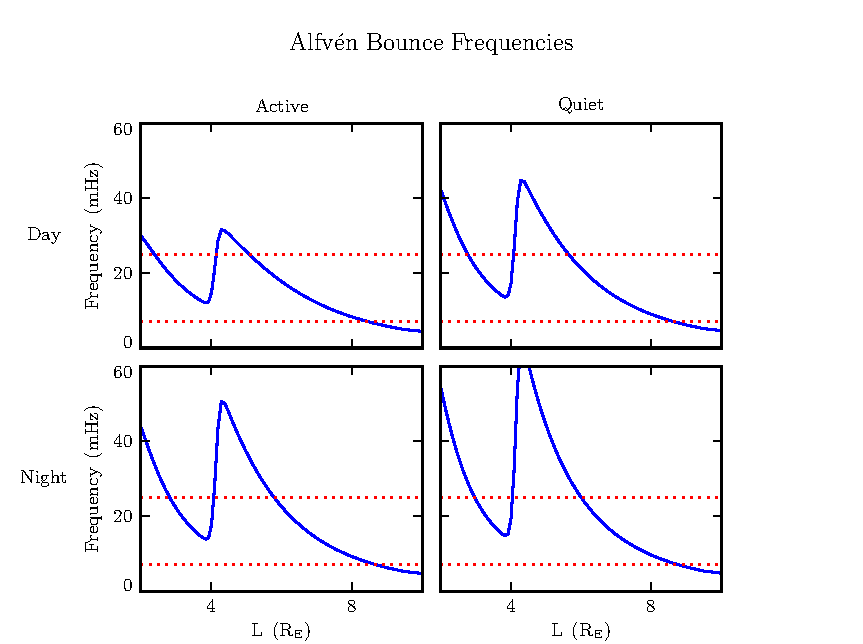
\includegraphics[width=\textwidth]{figures/fa.pdf}
  \caption[\Alfven Bounce Frequencies]{
    The above are bounce frequencies for an \Alfven wave moving back and forth
    along a geomagnetic field line. \Alfven speeds are computed based on
    profiles from Kelley\cite{kelley_1989}, as discussed in \cref{sec_profile}.
    Notably, the bounce frequency depends significantly on the position of the
    plasmasphere, taken here to be at $L=4$. Dotted lines indicate the Pc4
    frequency range: \SIrange{7}{25}{\mHz}. 
  }
  \label{fig_fa}
\end{figure}

In addition to being radially localized, FLRs in the Pc4 frequency band (also
called Pc4 pulsations, or just Pc4s) are localized in magnetic local time
(MLT\footnote{Noon points toward the Sun and midnight away from it, with 06:00
and 18:00 at the respective dawn and dusk flanks. }). They have also been shown
to occur preferrentially on the dayside, during storms or storm
recovery\cite{anderson_1990,dai_2015,engebretson_1992,kokubun_1989,liu_2009,
ukhorskiy_2005}. 

In the inner magnetosphere, the \Alfven frequency --- and thus the frequency of
FLRs --- often coincides with integer or half-integer\footnote{See
\cref{sec_harmonics}. } multiples of particle drift frequencies\cite{dai_2013}.
The resulting wave-particle interactions can give rise to significant
energization and radial diffusion of the particles. In some cases, the waves
also include an electric field parallel to the background magnetic field,
breaking the assumption that magnetic field lines are equipotential contours,
and contributing to the precipitation of energetic particles into the neutral
atmosphere\cite{goertz_1984,goertz_1979,thompson_1996,wygant_2002}. 

The present chapter introduces the structural characteristics of FLRs, how
those characteristics affect wave behavior, and several unresolved questions
related to that behavior. 

%\todo{The polarization of long-period \Alfven waves is rotated by \about\SI{90}{\degree} when passing through the ionosphere\cite{hughes_1974}. A wave that is azimuthally polarized in space is polarized north-south on the ground, and vice versa. It has been noted specifically that Pgs exhibit east-west polarized ground signatures\cite{takahashi_1992}. }

%\todo{Other planets\cite{glassmeier_2004}? Seems exciting but maybe not relevant. }

% -----------------------------------------------------------------------------
% -----------------------------------------------------------------------------
% -----------------------------------------------------------------------------
\section{Harmonic Structure}
  \label{sec_harmonics}

%\todo{Second-harmonic FLRs are unlikely to cause ground signatures\cite{takahashi_1992}. }

%\todo{Dai found a nice event\cite{dai_2013} that was unambiguously determined to be a fundamental-mode Pc4 in drift-resonant interaction with \about\SI{e5}{\eV} ions. Consistent with \cite{thompson_2001}. Other observations of odd harmonics: \cite{yang_2010,eriksson_2005}. }

Wave structure along a geomagnetic field line is indicated by harmonic number.
The first (or fundamental) harmonic has a wavelength twice as long as the field
line. The electric field perturbation is zero at the ionospheric foot points of
the field line, due to the conductivity of the ionosphere. For the first
harmonic, this puts an electric field antinode at the equator, along with a
node in the perpendicular\footnote{The parallel, or compressional, wave
magnetic field exhibits the same nodes and antinodes as the perpendicular
electric field\cite{radoski_1974}. } perturbation to the magnetic field. For
the second harmonic, the electric field has a third node at the equator, in
addition to the two at the ionospheric foot points, which is accompanied by an
antinode in the perpendicular wave magnetic field. \cref{fig_harmonics} shows a
qualitative sketch of the first and second harmonics: a series of snapshots in
time, in the rest frame of the wave. Perpendicular electric and magnetic field
perturbations are shown in blue and red respectively. 

\begin{figure}[!htb]
  \centering
  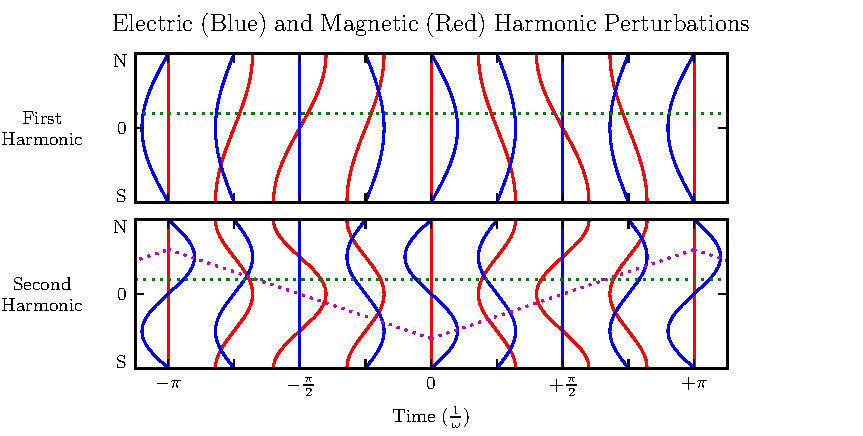
\includegraphics[width=\textwidth]{figures/harmonics.pdf}
  \caption[First and Second Harmonic Resonances]{
    The first (or fundamental) harmonic has an an antinode in its perpendicular
    electric field (blue) at the equator, along with a node in its
    perpendicular magnetic field perturbation (red). A single satellite can
    identify the first harmonic by the relative phase of the electric and
    magnetic field perturbations: an observer north of the equator (green) will
    see the magnetic field perturbation lead the electric field by
    $\pm\SI{90}{\degree}$. The second harmonic is the opposite: it has an
    electric field node at the equator, and an observer north of the equator
    will see the magnetic field perturbation lag the electric field by
    $\mp\SI{90}{\degree}$. Top and bottom signs correspond to the poloidal
    (shown) and toroidal polarizations respectively. The purple line sketches
    the path of a particle in drift-bounce resonance; in the particle's rest
    frame, the electric field is always to the right. 
  }
  \label{fig_harmonics}
\end{figure}

A first-harmonic FLR that is periodic or localized in the azimuthal direction
is conducive to drift-resonant wave-particle
interactions\cite{dai_2013,poulter_1983}. The particle is like a child on a
swing: whenever the path of the particle (or child) gets close to the wave
(parent), it gets a push, and always in the same direction. The wave fields
spend half its time pointing the other direction, just as the parent must shift
their weight backward to get ready for the next push, but at that point the
particle (child) is far away. 

Second-harmonic FLRs interact with particles through the drift-bounce
resonance, which is slightly more complicated. As the particle drifts
azimuthally, it also zig-zags north-south. The combination of those two
periodic motions must align with the phase of the wave electric field. An
example path is shown by the purple line in \cref{fig_harmonics}: the
particle's drift and bounce motions together ensure that it experiences a
rightward electric field throughout the wave's oscillation. 

The drift and drift-bounce resonance conditions is written,
respectively\cite{takahashi_2011}:
\begin{align}
  \omega - \azm \omega_D &= 0 &
  &\text{and}&
  \omega - \azm \omega_D &= \omega_B
\end{align}

Where $\omega$ is the frequency of the wave, $\omega_D$ and $\omega_B$ are the
particle's drift and bounce frequencies respectively, and \azm is the wave's
azimuthal modenumber, as discussed in \cref{sec_azm}. 

In principle, the first and second harmonics can be distinguished by their
frequencies, even from a single-point
observation\cite{anderson_1990,cummings_1969,green_1985}.  In practice,
however, this is not a reliable approach\cite{takahashi_2013}. Significant
uncertainties surround the mass density profile --- and thus the \Alfven speed
profile --- along a geomagnetic field line. 

Harmonic structure can also be deduced by noting the phase offset between the
wave magnetic field and its electric field (or the plasma
velocity)\cite{dai_2015,takahashi_1992}. In \cref{fig_harmonics}, the green
line indicates an observer just north of the magnetic equator. For a wave
polarized in the poloidal direction (see \cref{sec_polarization}), the observer
sees the electric field waveform offset from the magnetic field by a phase of
$\pm\SI{90}{\degree}$, where the top sign is for odd modes and the bottom sign
is for even modes. The signs are flipped for toroidally-polarized waves, and
again for waves observed south of the equator. 

In addition to a wave's parity, the phase indicates how energy is divided
between standing and traveling waves. Standing waves (phase of
$\pm\SI{90}{\degree}$) have a purely imaginary Poynting flux. Traveling waves
(phase of $\SI{0}{\degree}$ or $\SI{180}{\degree}$), on the other hand, have
real Poynting flux, indicating a net movement of energy. Wave lifetimes can be
estimated by comparing the energy density to the rate at which that energy is
carried away by Poynting flux, as is done in \cref{ch_rbsp}. 

Notably, the measurement of wave phase has only become viable with the advent
of satellites carrying both electric and magnetic field instrumentation, such
as THEMIS in 2007\cite{angelopoulos_2008} and the Van Allen Probes (formerly
RBSP, for Radiation Belt Storm Probes) in 2012\cite{stratton_2012}. 

Strictly speaking, the the phase offset of the electric and magnetic fields
does not provide the harmonic number --- only its parity. It's reasonably safe
to assume that an even mode is the second harmonic; the second harmonic is by
far the most commonly observed\cite{hughes_1978,singer_1982,takahashi_1990},
due in part to its excitement by the antisymmetric balloon
instability\cite{chan_1994,chen_1991,cheng_1994,southwood_1976}. However, the
distinction between the first and third harmonics is not always
clear\cite{chisham_1991,green_1985}; this issue is discussed further in
\cref{ch_rbsp}. Higher harmonics than that are not expected in the Pc4
frequency band. 

% -----------------------------------------------------------------------------
% -----------------------------------------------------------------------------
% -----------------------------------------------------------------------------
\section{Azimuthal Modenumber}
  \label{sec_azm}

The wavelength of an FLR in the azimuthal direction is indicated by its
azimuthal modenumber. A wave with modenumber \azm has an azimuthal wavelength
that spans $\frac{24}{\azm}$ hours in MLT. 

\begin{figure}[!htb]
  \centering
  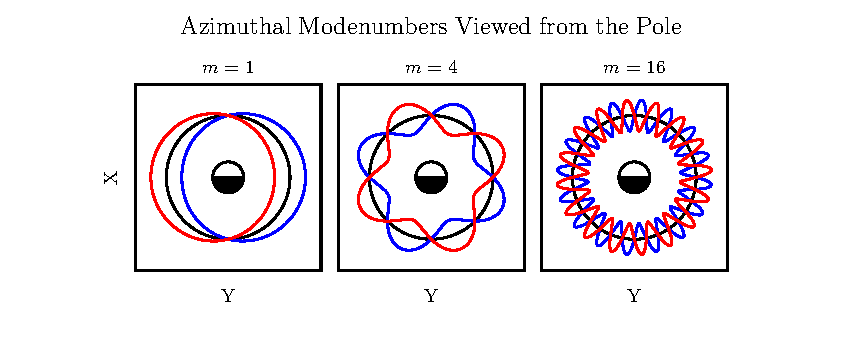
\includegraphics[width=\textwidth]{figures/azm.pdf}
  \caption[Azimuthal Modenumbers Viewed from the Pole]{
    Above are qualitative sketches of waves with azimuthal modenumbers 1, 4,
    and 16, projected into the ecliptic plane. Black circles show unperturbed
    fields, while the blue and red curves show perturbations. At $\azm = 1$,
    the wave is more or less a uniform displacement, while at $\azm = 16$
    azimuthal variations take place on spatial scales small compared to Earth's
    radius. 
  }
  \label{fig_azm}
\end{figure}

Waves with small azimuthal modenumbers ($0 < \azm < 10$) are typically driven
by broadband energy sources at the magnetosphere's boundary, such as variations
in the solar wind
pressure\cite{degeling_2014,hao_2014,kessel_2008,zong_2007,zong_2009}, sporadic
magnetic reconnection\cite{hughes_1994}, or Kelvin-Helmholtz waves on the
magnetopause\cite{chen_1974,liu_2011,southwood_1974}. In the low-\azm regime,
the shear and compressional \Alfven waves are coupled, which allows energy to
move across field lines until the driving frequency lines up with the local
\Alfven frequency\cite{lysak_1992}. Because of their broadband energy source,
low-\azm FLRs often have a mishmash of frequencies present in their
spectra\cite{dai_2015}, though the spectra are coherent in terms of
harmonic\cite{engebretson_1986}.

When the azimuthal modenumber is large (or, equally, when the azimuthal
wavelength is small), compressional propagation of \Alfven waves becomes
evanescent, so the movement of energy is guided by magnetic field
lines\cite{cummings_1969,radoski_1974}\footnote{Equally, the strength of a
wave's parallel component indicates its modenumber, a point which is revisited
in \cref{ch_results,ch_rbsp}. }. As a result, FLRs must be driven from within
the magnetosphere. Proposed energy sources include phase space gradients near
the plasmapause\cite{dai_2013}, particularly as the plasmasphere refills after
a storm or substorm\cite{engebretson_1992,liu_2013}. 

The atmosphere is known to attenuate waves with small spatial extent in the
perpendicular direction\cite{hughes_1976,wright_1999,yeoman_2001}. As a result,
FLRs may create no signature on the ground if their azimuthal modenumber is
large. For example, a recent paper by Takahashi shows a strong (\SI{2}{\nT} at
$L\sim10$), clear resonance with $|\azm|\gtrsim70$ and no corresponding ground
signature\cite{takahashi_2013}. 

Southwood\cite{southwood_1976} and Glassmeier\cite{glassmeier_1984} show that a
low frequency wave passing through the ionosphere on its way to Earth will be
attenuated per
\begin{align}
  \label{attenuation}
  \frac{B_E}{B_I} &= \frac{\Sigma_H}{\Sigma_P} \exp 
    \arg{ -\azm \frac{R_I - R_E}{R_E \sin \theta} }
\end{align}

Where $B_E$ and $B_I$ are the magnetic field strengths at $R_E$ (Earth's
surface, \SI{6783}{\km} geocentric) and $R_I$ (the ionosphere,
\about\SI{6900}{\km} geocentric) respectively. The integrated ionospheric
Pedersen and Hall conductivities, $\Sigma_P$ and $\Sigma_H$, are typically
within a factor of two of one another. Field lines near the plasmapause can
be traced to Earth at $\sin\theta\about0.4$. That is, by the time it reaches
the ground, the magnetic field from an FLR with $m=10$ is weaker by a factor
of two; at $m=100$, the factor is closer to 100. 

% -----------------------------------------------------------------------------
% -----------------------------------------------------------------------------
% -----------------------------------------------------------------------------
\section{Poloidal and Toroidal Polarizations}
  \label{sec_polarization}

%- One sentence paragraphs aren't
%- "Perhaps not coincidentally" Perhaps?
%- Fig. 3.4: I don't know how to read this plot. I guess the left is the first harmonic and the right is the second, but at first glance they looked the same. I guess I get it now...
%- Page 18 (page number not PDF number): You have half a sentence hanging on. You should probably make this images their own page.

Based on polarization, each FLR can be classified as either poloidal or
toroidal. The poloidal mode is a field line displacement in the meridional
plane, as shown in \cref{fig_poloidal}, with an accompanying electric field in
the azimuthal direction. The toroidal mode's magnetic displacement is
azimuthal, per \cref{fig_toroidal}; the associated electric field is in the
meridional plane. 

\begin{figure}[!htb]
  \centering
  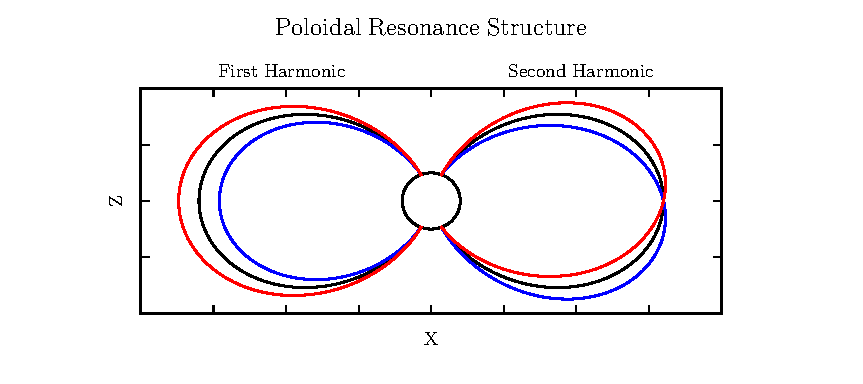
\includegraphics[width=\textwidth]{figures/poloidal.pdf}
  \caption[Poloidal Mode Structure]{
    The poloidal resonance is a magnetic field in the meridional plane. The
    displacement is radial near the equator, and can be accompanied by
    enhancement in the parallel magnetic field near the ionosphere. The first
    harmonic is shown on the left, and the second harmonic on the right. Lines
    are colored red and blue only to contrast with the unperturbed black field
    line. 
  }
  \label{fig_poloidal}
\end{figure}

\begin{figure}[!htb]
  \centering
  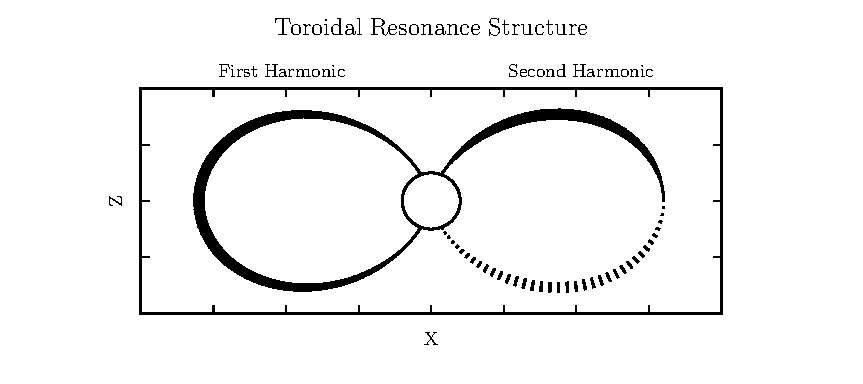
\includegraphics[width=\textwidth]{figures/toroidal.pdf}
  \caption[Toroidal Mode Structure]{
    A toroidally-polarized FLR has a magnetic perturbation in the azimuthal
    direction, as shown. Bold lines are taken to be above the page, and dotted
    lines below the page, with the displacement indicated by the line's width.
    The first harmonic --- where the entire field line oscillates in and out of
    the page --- is shown on the left. The second harmonic is on the right,
    with northern and southern halves perturbed in opposite directions. 
  }
  \label{fig_toroidal}
\end{figure}

Both poloidal and toroidal waves are noted for their ability to contribute to
the energization and radial diffusion of trapped particles. The poloidal mode
interacts more strongly, since its electric field is aligned with the trapped
particles' drift motion. Poloidally-polarized waves are also more prone to
creating magnetic signatures on the ground, due to ducting in the
ionosphere\cite{fujita_1988,greifinger_1968}. 

Toroidal modes have been shown to outnumber poloidal modes\cite{anderson_1990}.
Perhaps not coincidentally, poloidally-polarized waves rotate asymptotically to
the toroidal mode\cite{mann_1995,mann_1997,radoski_1974}. Poloidal waves with
low azimuthal modenumber --- such as those driven by broadband sources at the
magnetopause --- rotate on timescales comparable to their oscillation periods.
The two modes are also coupled directly by the ionospheric Hall
conductivity\cite{kato_1956}. 

The eigenfrequencies for poloidal and toroidal FLRs are similar, though not
identical\cite{green_1985}. It has furthermore been noted that
toroidally-polarized waves exhibit a strong relationship between frequency and
$L$-shell (or latitude), while poloidal waves at fixed frequency are spread
more broadly in $L$\cite{engebretson_1986}. 

%\todo{Fishbone instability\cite{chen_1984,mcguire_1983}. Like the poloidal mode, but for lab plasmas. }

%\todo{Poloidal and toroidal modes are coupled by the ionospheric Hall conductivity\cite{kato_1956}. The Hall conductivity also increases the ``ringtime'' of these resonances, allowing them to oscillate through the inductive process rather than be dissipated as Joule heating\cite{waters_2013}. }

%\todo{Toroidal modes show a clear frequency dependence with $L$. Poloidal modes less so. Citation... \cite{engebretson_1986}? }

% -----------------------------------------------------------------------------
% -----------------------------------------------------------------------------
% -----------------------------------------------------------------------------
\section{Giant Pulsations}

%- What's special about Tromso Norway? I feel like you need half a sentence more!

The study of geomagnetic pulsations long predates satellites, sounding rockets,
or even the word ``magnetohydrodynamics''\footnote{The term was first used by
\Alfven in the 1940s\cite{alfven_1946}. }. Large, regular oscillations in the
magnetic field were noted as early as 1901\cite{birkeland_1901}. Eventually,
the term ``giant pulsation,'' or Pg, arose to describe such pulsations. 

On the ground, Pgs are notable for their strikingly sinusoidal waveforms,
their eastward drifts, and their specific occurrence pattern: Pgs are typically
seen pre-dawn, at latitudes of \SIrange{60}{70}{\degree}. Pgs generally fall
into the Pc4 frequency band\footnote{The Pc4 range is periods of
\SIrange{45}{140}{\s}, while Pgs range from
\SIrange{60}{200}{\s}\cite{brekke_1987}. }. Their harmonic structure was a
source of controversy for decades, but recent multisatellite observations seem
to be in agreement that they are odd harmonics, probably
fundamental\cite{glassmeier_1999,hillebrand_1982,kokubun_1980,kokubun_1989,
takahashi_2011,takahashi_1992}. They are poloidally polarized, with modenumbers
$10 \lesssim \azm \lesssim 40$\cite{glassmeier_1980,hillebrand_1982,
poulter_1983,rostoker_1979,takahashi_1992}. 

Whereas FLRs are waves in space which may produce ground signatures,
``giant pulsation'' refers to the ground signature
specifically\footnote{Historically, the wave designations shown in
\cref{tab_iaga} all referred to ground phenomena. Over time, they have come to
describe satellite observations as well, including those without corresponding
signatures on the ground. }. That is, Takahashi's satellite observation of a
sinusoidal, morningside, high-\azm, fundamental poloidal resonance was not
classified as a Pg because it did not produce a signal on the
ground\cite{takahashi_2013}. 

%\todo{Pgs are localized to within \SIrange{2}{5}{\degree} in latitude\cite{motoba_2015,takahashi_2011,veldkamp_1960}. }

%  --- half of them measured at Troms{\o}, Norway

Due to their remarkably clear waveforms, Pgs are typically found by ``visual
inspection of magnetometer data''\cite{motoba_2015}. Over the course of the
past century, a number of multi-year (sometimes multi-decade\cite{brekke_1987})
surveys have totaled nearly one thousand Pg events. On average, a ground
magnetometer near \SI{66}{\degree} magnetic latitude observes \about10 Pg
events per year\cite{brekke_1987,harang_1941,rolf_1931,sucksdorff_1939}.
Observations are not distributed uniformly; rather, giant pulsations are most
common near the equinox and during times of low solar activity. 

Unlike Pc4 pulsations in general, Pgs show no particular correlation with storm
phase\cite{motoba_2015}. However, they do often occur as the magnetosphere
recovers from a substorm\cite{motoba_2015,rostoker_1979}. 

% -----------------------------------------------------------------------------
% -----------------------------------------------------------------------------
% -----------------------------------------------------------------------------
\section{Motivations for the Present Work}

A great deal has been learned --- and continues to be learned --- through
observations of field line resonance. However, the cost-to-benefit ratio is
climbing. As summarized in the sections above, FLR behavior depends
significantly on harmonic structure, azimuthal modenumber, and polarization ---
not to mention frequency, spectral width, and so on. With each degree of
freedom comes the necessity for an additional simultaneous observation. 

Similarly, as FLRs have been shown to depend on ever-more-specific
magnetospheric conditions, analytical techniques have fallen out of favor. The
height-resolved ionosphere, multidimensional \Alfven speed profile, and
inconvenient geometry combine to create a problem beyond the reasonable purview
of pencil and paper. 

That is, the topic of field line resonance is ripe for numerical modeling. 

Past models of the magnetosphere have been limited in their consideration of
FLRs. Reasons include overly-simplified treatment of the ionospheric boundary,
no consideration of the plasmapause, limited range in \azm, and the inability
to compute ground signatures. \cref{ch_model} presents a model which addresses
these issues, allowing the computation of field line resonance with
unparalleled attention to realism. 

The model allows a bird's-eye view of the structure and evolution of FLRs. As
such, not only can several open questions be addressed, but their answers serve
to unify a number of seemingly-disparate properties described in the sections
above. 

The rotation of poloidally-polarized waves to the toroidal mode is
investigated. Particular attention is paid to the importance of azimuthal
modenumber and ionospheric conductivity. The interplay between said rotation
and the transport of energy across field lines --- which also depends on
azimuthal modenumber --- is considered as well. 

By their nature, drifting particles have the potential to spur wave-particle
interactions at all MLT. However, Pc4 observations are strongly peaked on the
dayside. In a 2015 paper, Dai notes, ``It is not clear why noncompressional
[high-\azm] Pc4 poloidal waves, which are presumably driven by instability
within the magnetosphere, preferrentially occur on the
dayside''\cite{dai_2015}. Motoba, later that year, echoes, ``It is unclear
whether other generation mechanisms of fundamental standing waves ... can
explain the localization of Pgs in local time''\cite{motoba_2015}. This, too,
is considered numerically: to what degree is field line resonance affected by
the (day-night asymmetric) conditions of the ionosphere? 

An attempt is also made to demystify giant pulsations. It's been shown that
toroidal Pc4s outnumber poloidal ones, and that most poloidal Pc4s are even, so
perhaps it should come as no surprise that (poloidal, odd) Pgs are rare. Is it
truly the case that Pgs are only ``a small subset of fundamental poloidal
waves''\cite{takahashi_2013}, set apart from the rest by their distinctive
properties? Or, said another way, to what degree do the properties
associated with Pgs arise in fundamental poloidal waves overall? 

%It's been shown that a ground magnetometer \SI{66}{\degree} north of the magnetic equator observes \about10 Pg events per year. It's also been shown that poloidal Pc4s are rare compared to toroidal ones, and that most poloidal Pc4s are even harmonics. However, little attention has been paid to how these rates line up with one another. Given the relative occurrence rate of poloidal and toroidal waves, of odd and even harmonics, and of diffuse and sharp spectral peaks, just how unusual are giant pulsations? 


%The present work uses a numerical model to investigate the preferrential occurrence of field line resonances in the Pc4 range --- particularly first-harmonic poloidal modes, such as giant pulsations --- in MLT. 

%Giant pulsations are commonly referred to as ``rare''\cite{brekke_1987}, or even ``a small subset of fundamental poloidal waves''\cite{takahashi_2013}. However, quantification of Pg occurrence --- compared to the occurrence rate of fundamental poloidal Pc4s in general --- is thin on the ground. It's been shown that poloidal Pc4s are rare compared to their toroidal counterparts. It's also been shown that, among poloidal Pc4s, the second harmonic is the most common. 


% Dai writes, in his 2015 paper\cite{dai_2015}, ``It is not clear why noncompressional [high-\azm] Pc4 poloidal waves, which are presumably driven by instability within the magnetosphere, preferrentially occur on the dayside.'' 

% Motoba\cite{motoba_2015}, similarly, notes ``It is unclear whether other generation mechanisms of fundamental standing waves ... can explain the localization of Pgs in local time.''

% Giant pulsations have variously been referred to as ``intriguing''\cite{green_1985}. ``rare''\cite{brekke_1987}, even to the point of being ``a small subset of fundamental poloidal waves''\cite{takahashi_2013} --- note that it's well known that fundamental poloidal mode waves are already rare in comparison to second harmonic waves. 

%\todo{What's going on with the MLT localization of Pc4 pulsations? Is there something spooky going on with the driving? Maybe the ionosphere just kills FLRs on the nightside! }

%\todo{What's so special about Pgs? How rare are they, really, compared to fundamental poloidal modes in general? How does that line up with the occurrence rate of nice, sinusoidal waveforms in second-harmonic Pc4s? That is, is there something special about Pgs, or do they just live in a ``sweet spot'' with respect to constraints on observation and resonance? }

%\todo{Parallel electric fields. In this regime, we're looking at inertial effects, not kinetic effects\cite{goertz_1979,thompson_1996}. Should produce non-monoenergetic precipitation, which are observed\cite{goertz_1984}. Consistent with MHD models\cite{chaston_2000,chaston_2002}. Inertial-scale structures observed with Polar\cite{wygant_2002}. }

%\todo{The plasmapause matters! Effective potential well, analogous to \Schrodinger's equation\cite{lee_1998,lee_1999,dai_2009}. Shown in theory\cite{klimushkin_1998,leonovich_2000,klimushkin_2004,mager_2013} and in observation\cite{takahashi_2009,takahashi_2010}.  }

%\todo{All sorts of FLR occur preferrentially (though not exclusively) on the dayside\cite{dai_2015,ukhorskiy_2005}. }

%\todo{Any waves with frequencies of $\SIrange{e-3}{1}{\Hz}$ are termed ULF waves --- ultra low frequency. ULF waves are furthermore categorized in terms of their morphological characteristics. Pc waves are continuous (exhibiting a fairly consistent waveform over a large number of wave periods) while Pi are irregular; the waves are further partitioned into frequency bands. See \cref{tab_iaga}. }

%\todo{These are Jacobs' original ranges... but are they really reflective of the jargon still used? It's weird that these ranges bottom out so far below 1000s. }

%\todo{While the IAGA characterizations are based on wave morphology, they do a decent job of deliniating between the different underlying physical processes as well. Pi2 pulsations (irregular waves with periods of a minute or two) tend to be excited on the nightside; they are associated with substorm onset (though the processes that give rise to Pi2s --- and their relation to substorm onset --- remains controversial). Pc1 and Pc2 pulsations tend to be EMIC (electromagnetic ion cyclotron) waves near the ion gyrofrequency, which are important for the precipitation of electrons (?). }

%Pi2: ``Clearly linked to substorm disturbances and other impulsive dynamics are the irregularly shaped waves in the 7--25-mHz band referred to as Pi2. Recent work on these waves suggests that their periodicity reflects the spectrum of global mode excitations of the plasmasphere but there is a competing proposal that the dominant frequencies are imposed by the modulated flows in the magnetotail.''\cite{kivelson_2006}

%\todo{The present work is specifically concerned with field line resonances near the plasmapause. These waves fall in the Pc4 range, with frequencies around \SI{10}{\mHz}\footnote{Notably, field line resonances can also fall within the Pc3 and Pc5 ranges. }. }

% Less than a decade later, Sigura presented observational evidence of the phenomenon: a wave seen simultaneously at the northern and southern foot points of a geomagnetic field line\cite{sigura_1961}. 

%\todo{There's no discussion of ULF frequency bands, or even use the term ``Pc4.'' That's probably a problem. Introduce \SIrange{7}{25}{\mHz}! }

% \todo{Pc4s are localized in L and in MLT\cite{anderson_1990,dai_2015,engebretson_1992,liu_2009}. Near the plasmapause. This is an important part of why the 2.5D model is a good fit! }

% \todo{Drift resonance with azimuthal wavenumber. In the analogy of a parent pushing a child on the swing, the child still gains energy even if the parent only shows up half the time. Or Are there a bunch of parents? The analogy starts to fall apart past there. }

%``To summarize, the general buffetting of the magnetosphere by variations in the solar wind dynamic pressure, or perhaps by sporadic magnetic reconnection, provides a broad band energy source to the magnetosphere. The magnetospheric cavity as a whole rings at its own eigenfrequencies, thus transporting energy at just those frequencies to field lines deep in the magnetosphere. Those field lines whose eigenfrequencies match one of the cavity eigenfrequencies couple to the cavity mode and resonate strongly, producing the classical field line resonance signature.\cite{hughes_1994}'' 

% Compressional driving doesn't preclude drift or drift-bounce resonance\cite{zong_2007,zong_2009}. 

% The strength of the compressional-poloidal coupling indicates \azm\cite{hughes_1994}. 

% Low-\azm waves tend to be more muddled... driven by broadband sources rather than resonance\cite{dai_2015}. 

% Small structures are also damped; resonances narrower than $\sim \SI{100}{km}$ aren't visible on the ground. See also Glassmeier and Stellmacher, 2000 (about small latitude). \Alfven waves with small latitudinal scale\cite{glassmeier_2000} are screened by the ionosphere. Attenuation factor from \cite{hughes_1976} and \cite{glassmeier_1984}. 

%``Pgs maybe a manifestation of a small subset of fundamental poloidal waves excited in the magnetopause.'' \cite{takahashi_2013}

%``It is not clear why noncompressional [high-\azm] Pc4 poloidal waves, which are presumably driven by instability within the magnetosphere, preferrentially occur on the dayside.\cite{dai_2015}''

%``It is unclear whether other generation mechanisms of fundamental standing waves such as drift wave instability\cite{green_1979} can explain the localization of Pgs in local time (LT).''\cite{motoba_2015}

% Shear mode incident on the ionosphere, pederson current closes FAC, Hall current then generates a fast mode wave which may be detected in space or on the ground\cite{tamao_1965}. 

% Poloidal and toroidal ULF polarizations are treated differently by the ionosphere\cite{greifinger_1968} (more recently, \cite{fujita_1988}) due to ducting by the ionosphere. 

% In the example shown of a fundamental mode poloidal Pc4, and in the example of a higher harmonic Pc4, a mishmash of toroidal activity is present. \cite{dai_2015}, figure 8 and 9 respectively. 

% Observations of odd-mode poloidal waves... possible fundamental\cite{yang_2010,eriksson_2005}.

% \todo{Do the unambiguous Pc4 events in \cite{takahashi_2011} and \cite{dai_2013} also have a mishmash of toroidal activity? NO. }

% Poloidal Pc4s occur primarily during geomagnetically active times\cite{dai_2015}. This confirmed and refined older work\cite{engebretson_1987}. 

% Drift resonance happens when the bounce frequency of an \Alfven wave between the northern and southern ionospheres matches the bounce frequency of nearby particles. It allows the energization of ring current and radiation belt particles through drift and drift-bounce resonance\cite{elkington_1999,mann_2013,ozeke_2008,southwood_1976}. By multiple wave-particle interactions, poloidal ULF waves [FLRs] can lead to radial diffusion of radiation belt particles\cite{elkington_2003,ozeke_2012,tu_2012}.

%\begin{figure}[!htb]
%    \centering
%    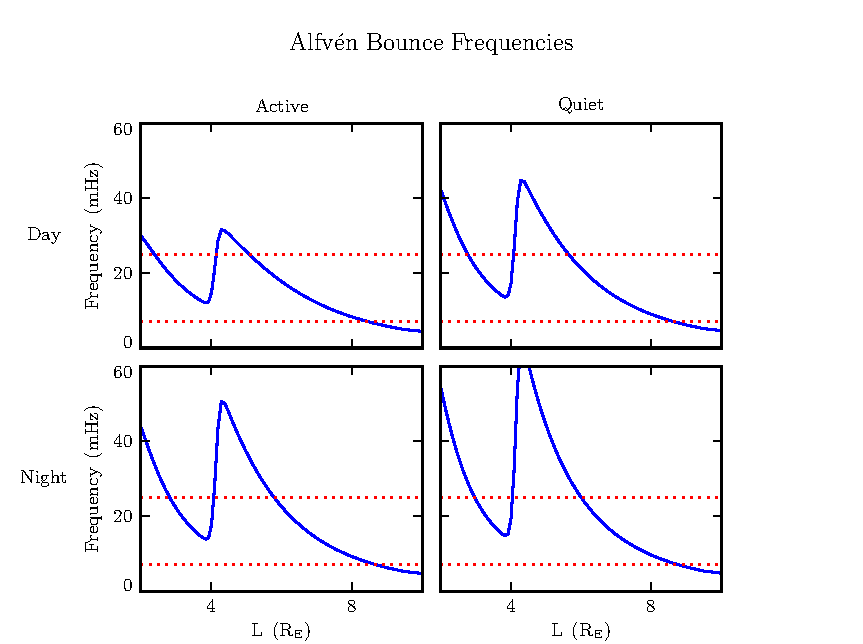
\includegraphics[width=\textwidth]{figures/fa.pdf}
%    \caption[\Alfven Bounce Frequency Profiles]{
%      \Alfven bounce frequency profiles, computed by integrating the the \Alfven speed back and forth over a field line. $f_A = \lrb{ \oint \frac{dz}{v_A} }^{-1}$. Dotted lines indicate the Pc4 frequency range, \SIrange{7}{25}{\mHz}. In each profile, the effect of the plasmapause is clearly visible, centered at $L=4$. Field lines just inside and just outside the plasmapause appear susceptible to resonance in the Pc4 band. \todo{Talk about how the size of the plasmasphere can be adjusted, and \SI{4}{\RE} is just a typical value. }
%    }
%    \label{fig_fa}
%\end{figure}

% ULF waves have been shown to correlate with pulsating aurora and with chorus\cite{jaynes_2015}. It's believed that (in the case presented) substorm injection drove Pc4-5 pulsations, which modulated chorus waves, which pitch-angle scattered electrons with energies on the order of \SI{10}{\kilo\eV}. 

% \todo{Theoretical consideration of decay vs propagation, by frequency. Lysak and Yoshikawa 2006. }

% Drift-wave instability\cite{hasegawa_1971,green_1979,green_1985} is also a possibility for exciting fundamental poloidal waves, though it requires cold plasma, so it could only happen in the plasmasphere. 

% AMPTE/CCE data has shown a correlation between poloidal Pc4 activity and intense ring current flux near the equator\cite{engebretson_1988}. 

% Toroidal mode is usually associated with external driving\cite{chen_1974,southwood_1974}. 

% A Hall-conducting ionosphere reflects ULF waves\cite{hughes_1974}. 

% Compressional poloidal Pc4 pulsations are much more common during storms, but not particularly sensitive to storm phase. Noncompressional ones occur primarily during recovery\cite{dai_2015,rostoker_1979,engebretson_1992,anderson_1994}. Note that Dai\cite{dai_2015} was pretty generous about what counted as a storm... anything that hits \SI{-30}{\nano\tesla}. So \cite{motoba_2015} may not have counted the same way when they found no particular correlation with storm phase. 

%\todo{First Pg observation\cite{birkeland_1901}. }

%\todo{Pgs are most common during solar minimum, perhaps because of decreased mass loading of heavy ions\cite{denton_2011}. }

%\todo{The harmonic structure of giant pulsations was once controversial; at this point, there is general consensus (based on satellite data) that they are fundamental poloidal modes\cite{glassmeier_1999,hillebrand_1982,kokubun_1980,kokubun_1989,takahashi_1992,takahashi_2011}. }

%\todo{Giant pulsations observed on the ground tend to have azimuthal modenumbers $10 \lesssim \azm \lesssim 40$\cite{glassmeier_1980,hillebrand_1982,poulter_1983,rostoker_1979,takahashi_1992}. }

%\todo{Giant pulsations peak around \SI{66}{\degree} MLAT\cite{motoba_2015}, corresponding to L=6, but have been observed at $5 \lesssim L \lesssim 7$\cite{green_1985}. Most prevalent on the morningside, with some in the afternoon. }

% Another past study: \cite{takahashi_1984_spectrum}. Satellite data is surveyed and classified by polarization, harmonic, wavenumber, etc, in order to determine the mechanisms for generating \Alfven waves. Old, but still pretty representative, according to Motoba\cite{motoba_2015}. 

% A long-period \Alfven wave passing through the ionosphere is rotated by about 90 degrees\cite{nishida_1964_screening,hughes_1974}. That would translate a poloidal resonance in space to an east-west ground signature. 

% \cite{motoba_2015} suggests that Pgs originate from the fundamental poloidal mode waves at all local times. 

% It seems to be the convention to find a Pg event on the ground, then look at satellite data. That's certainly what was done in \cite{motoba_2015}. 

% Per \cite{motoba_2015}, most Pg events happen around $L=7$, but some do happen near the plasmapause, as seen(?) by \cite{green_1985}. 

% ``The AL distribution shown in Figure 14c are consistent with the findings of \cite{rostoker_1979} that Pgs occur as the magnetosphere recovers from previous activities (substorms).''\cite{motoba_2015} Finds this to be reasonable because it's ``very likely'' that energetic ions injected into the inner magnetosphere from the magnetotail provide energy to Pgs. 

% Analysis of GOES data from 2008 to 2013 shows about 100 Pg events. They are concentrated on the morningside. No particular correlation with storm phase\cite{motoba_2015}. 

% Recall compressional poloidal Pc4s are mostly during storm time, and noncompressional are mostly specifically during late recovery\cite{dai_2015}. Only 19 fundamental poloidal mode examples were identified from the 390 noncompressional poloidal events. 

%
% From W J Hughes' Magnetospheric ULF Waves: A Tutorial With a Historical Perspective
%

% rolf 1920 for early observation of Pi2

% Patel 1965 made observations in space, and matched them to observations on the ground
% Cummings et al 1969 numerically integrated Dungey's equations to estimate eigenfrequencies
% soviets discovered that different pulsations have different sources in the 1970s; see troitskaya 1993 and greenstadt and russell 1993
% troitskaya 1969 showed that Pc3 can sometimes be explained by a sudden change in the size of the magnetosphere following an impulse. an example --- this must have also been seen earlier. because... 
% Bolshakova and Troitskaya 1968 showed that Pc3 observation depends on IMF N/S. Iff IMF is within about 50 degrees of the earth-sun linem Pc3 is observable on the ground. 
% Troitskaya et al 1971 showed Pc3 frequencies at L=3 depend on IMF magnitude
% Gul'elmi 1974 and Kovner et al gave theoretical justification for these observations. 
% Russell and Hoppe 1981 made observations upstream of the bow shock to unify some ideas. upstream waves are driven by ion cyclotron instability, which depends on IMF magnitude. 

% Gringauz et al 1970 found that solar wind number density affects Pc3 and Pc4 periods (oppositely). The Pc4 effect is a standing question. 

% Samson et al 1971 new observations with digital recording and arrays near the plasmapause! they showed MLT dependence of peak amplitude, and different regions of opposite circular polarization. 
% Dungey 1954 had suggested KH as a wave energy source, which explained the flipping circular polarization at noon. 
% Southwood 1974 went back to the equations and came up with a reason for resonance. waves hitting the bow shock propagate in as an evanescent fast mode. when it gets to a resonant field line, the fast mode couples to the shear mode. the energy tunnels. this only happens if dissipation is finite. 
% Chen and Hasegawa 1974 did too, independently
% Newton et al 1978 showed that joule dissipation at the ionosphere is dominant, and that the amount of dissipation determines the width of the resonance. 

% kivelson et al 1984 argued for cavity mode eigenfrequencies. Pc5. 
% kivelson and southwood 1985, 1986 did analytical work to defend it. 
% Lee and Lysak 1991 did numerical work in a dipole geometry. 

% Harrold and Samson 1992 The waves probably have to be reflected by the bow shock, not by the magnetopause, to line up with the observed eigenfrequencies. 1 to 3 mHz. 

% allan et al 1985 did early observation of ULF waves (Pc5 and Pc4) from waveform plots. 
% Waters et al 1991 ground-based observation of Pc3 and Pc4 before spacecraft existed at small L. 
% Menk et al 1993 also


